\section{Test of MIT Detector}
After populating the boards with all of the electronic components, each connection was checked using a multi-meter. The DC-DC Booster connection on the main PCB was tested without the SiPM PCB (See Figure \ref{Bias Voltage check}) and found to have to correct biasing voltage required, confirming that all the components of the main PCB are correctly soldered, and the detector is ready for assembly.

    From plugging in the constructed detector, the OLED screen appears, signifying it is running.  Every 5.8 \textmu s measurements are recorded, which is longer than the length of the peak detector pulse; therefore, the initial few measurements appear constantly and are excluded when analyzing muon counts. The trigger pulse time has an uncertainty of 0.4 \textmu s, and using the laptop for readout adds an additional uncertainty of 0.1 ms. 

    Measurements were conducted in the basement of the Natural Science Center at GSU, and the rate of muon counts per second was found to be 0.5 +/- 0.007. When the detector was taken outside for measurements, the rate of muon counts increased by a factor of 2. These results are consistent with what we expected; however, the dead time for both ranged from 1,000-55,000 ms. An appropriate dead time would be less than 1,000 ms. Therefore, further modifications will be needed to decrease the time it takes the Arduino to perform tasks prompted by the code before testing the detector's efficiency against the cosmic ray muon telescope. 

    To accurately obtain significant data to test the detector's performance, we will need to eliminate the effects of atmospheric pressure and record data for seven days or more. The current code does not include a function to save the output to a text file,  deleting measurements displayed through a terminal window as time progresses. This poses a difficulty on consistently recording data for the appropriate length of time.  Therefore, additional modifications on the detector are needed as well. 
\begin{figure}[htb]
\centering
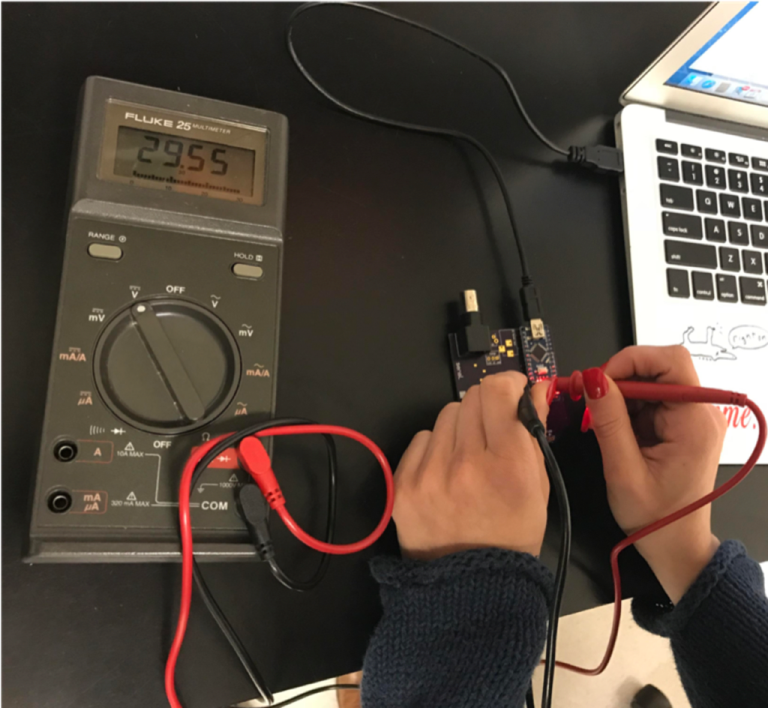
\includegraphics[width=0.75\textwidth]{images/VoltageReading.png} 
\caption{Biasing voltage being check by connecting a multi-meter between the HV pin and ground of the 6-pin header on main PCB.}
\label{Bias Voltage check}
\end{figure}
\begin{figure}[htb]
\centering
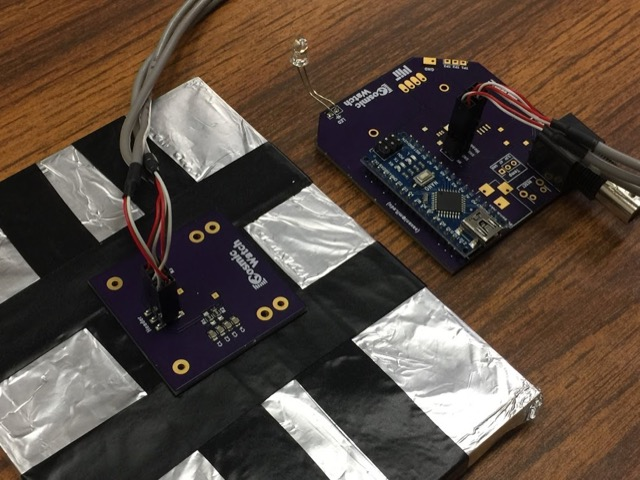
\includegraphics[width=0.75\textwidth]{images/Connection_PCB.jpg} 
\caption{Connection of the six-pin header on the SiPM PCB to the six-pin connector on the main PCB using electrical wires is shown prior to wrapping the scintillator and SiPM PCB light tight with electrical tape.}
\end{figure}